\chapter{Literature Survey}

In this section, we present the ITracker neural network introduced by \cite{MIT_EyeTracking_paper} used as our base model. We then discuss the extractors explored to extract the face and eyes required as inputs to the network. We also compare the performance of these face detectors surveyed in this work for the purpose of redaction.


%%%%%%%%%%
\section{ITracker Neural Network}
The ITracker Neural Network proposed by \cite{MIT_EyeTracking_paper} is a deep CNN that takes the face and eye crops and a face grid as inputs and predicts the XY gaze coordinates on the screen w.r.t. the camera as output. The X-coordinate and Y-coordinate axes are oriented rightwards and upwards, respectively, with the camera located at the origin of this reference frame. We leverage this model for our purposes of classification of gaze (2-Way or 3-Way) by replacing the final XY gaze regression layer with a gaze classification layer to output the gaze class labels.

\begin{figure}[h]
  \centering
    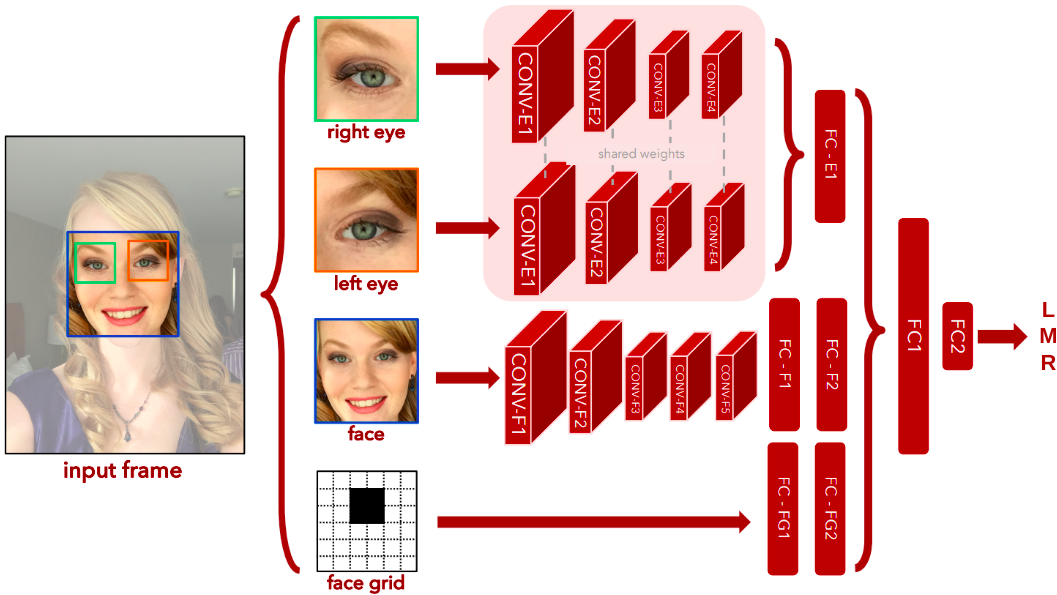
\includegraphics[width=1.0\textwidth]{LiteratureSurvey/ITrackerNN}
    \caption[ITracker NN]{ITracker NN for Gaze Classification}
    \label{fig:iTrackerNN} 
\end{figure}

The crops of the face and eyes are extracted from the frame by an extractor. In this work, we first use The Histogram of Oriented Gradients (HOG) face extractor provided in the Dlib library of OpenCV and RetinaFace detector for extracting face and eyes. As we explore other face detectors in the upcoming sections, we compare these and finally arrive at the best detector out of these detectors for extracting face and eyes. The face grid input to the neural network is a binary mask of the face in the entire frame.


%%%%%%%%%%
\section{S3FD: Single Shot Scale-invariant Face Detector}
S3FD is based on the state-of-the-art SSD object detection framework \cite{ssd2016} where, unlike the detection and classification module, which occurs at the end of the architecture pipeline in a Region Proposal Network, the detection and classification are performed at various levels of feature maps. As depicted in figure \ref{fig:s3fdNN}, the shallow feature map has a small receptive field, which is responsible for and drastically improves the detection of small-scale faces. On the other hand, the deep feature map has a large receptive field, which is responsible for the detection of large-scale faces. 

\begin{figure}[h]
  \centering
    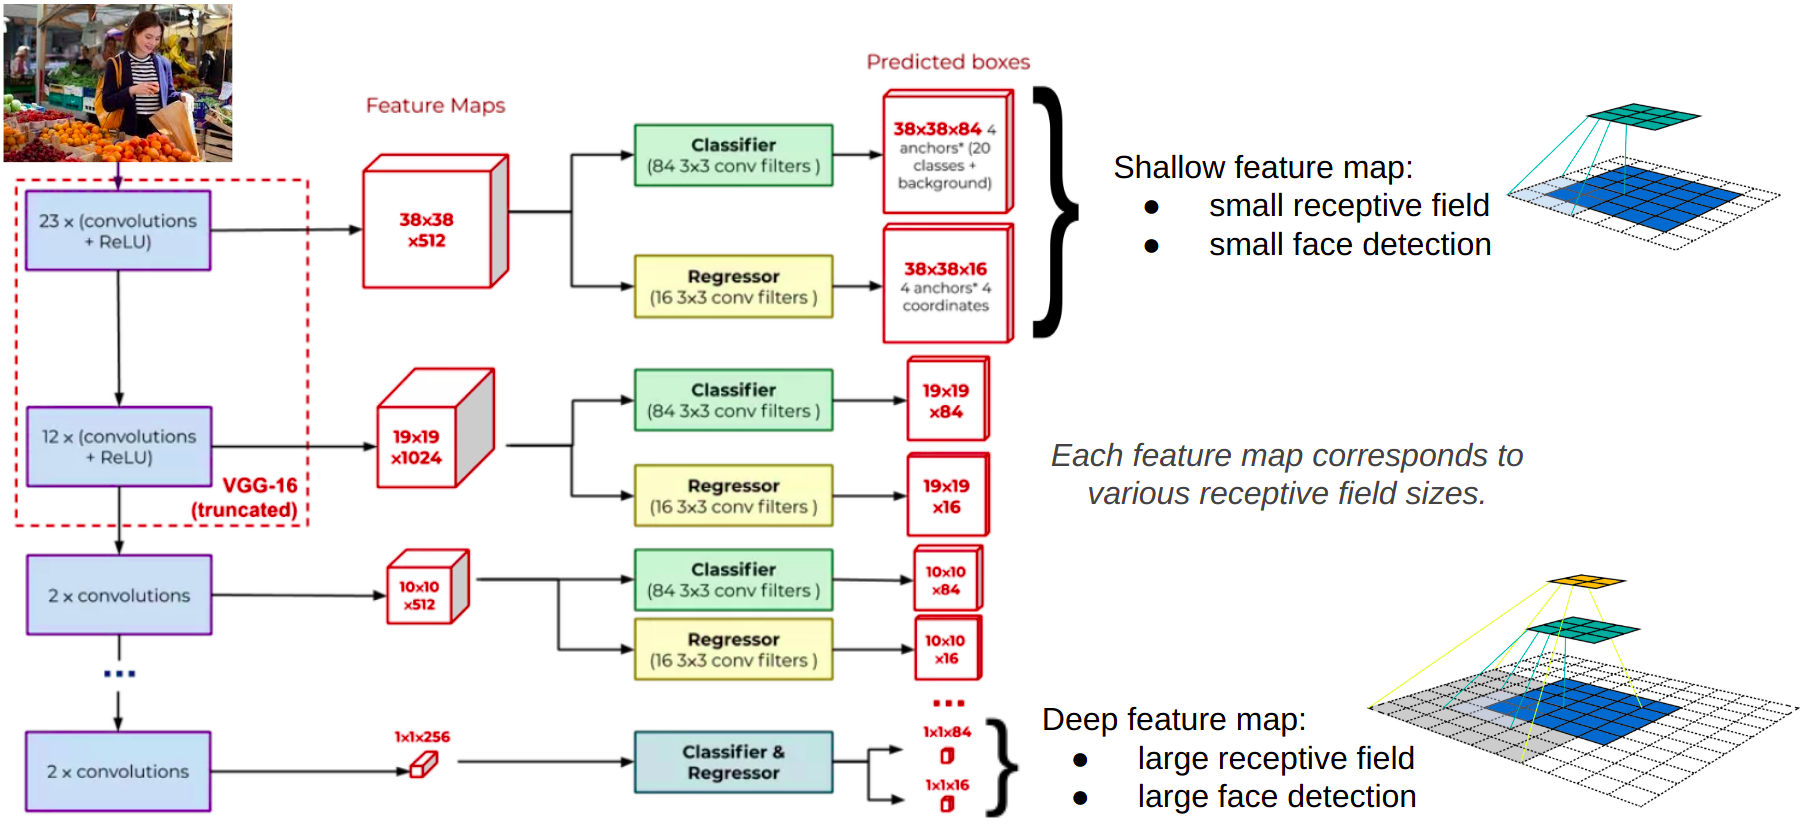
\includegraphics[width=1.0\textwidth]{LiteratureSurvey/S3FD_NN}
    \caption[S3FD]{S3FD NN Architecture}
    \label{fig:s3fdNN} 
\end{figure}

\paragraph{Designing Anchor Scale}
In addition to the scale-invariant detection framework discussed above, the anchor scales at different levels of feature maps are designed on the basis of Effective Receptive Field (ERF) at that level, as shown in figure \ref{fig:anchorScaleERF}. The reasoning is that the ERF is the region in the input image, which significantly affects the detection at a particular level. So, designing anchor scales that correspond to the ERF scale helps to improve the detection rate. 

\paragraph{Max-out Background label}
Although the framework of detection at various levels of the feature map imparts scale-invariance to the network, a problem arises due to the first detection layer, as shown in figure \ref{fig:maxOutBgLabel_problem}. Due to a large number of background labels at small-scaled anchors, the face detection task gets exposed to an extremely unbalanced binary classification task and the overall false-positive rate increases for small faces.

In order to reduce the false-positive rate for small faces, the proposed solution is to predict \emph{N} scores for the background label for each anchor in the first detection layer and then select the highest score as the confidence of the background label (figure \ref{fig:maxOutBgLabel_solution}).

\begin{figure}[h]
    \centering
    \captionsetup[subfigure]{justification=centering}
    \subfloat[Designing Anchor Scale from ERF]{{
        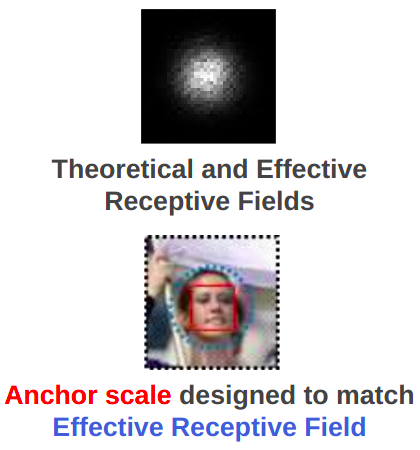
\includegraphics[scale=0.25]{LiteratureSurvey/AnchorScaleERF}
        \label{fig:anchorScaleERF}
        }}
    \quad
    \subfloat[Unbalanced Binary Classification]{{
        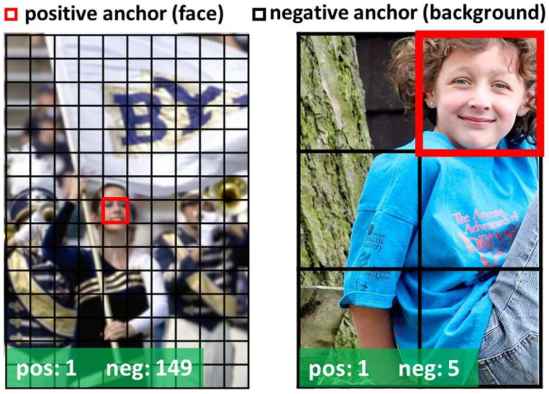
\includegraphics[scale=0.25]{LiteratureSurvey/MaxOutBgLabel_problem}
        \label{fig:maxOutBgLabel_problem}
    }}
    \quad
    \subfloat[Max-out Background Label]{{
        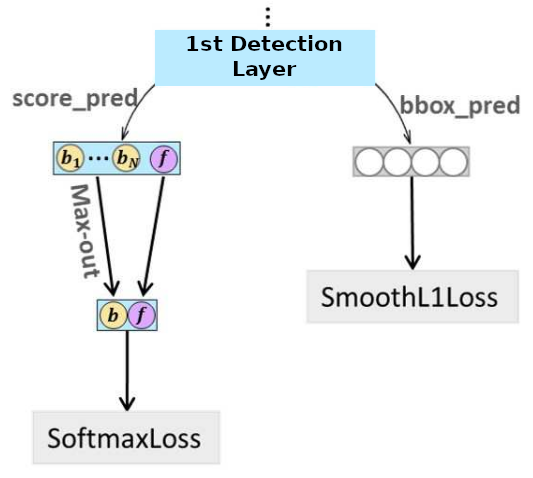
\includegraphics[scale=0.25]{LiteratureSurvey/MaxOutBgLabel_solution}
        \label{fig:maxOutBgLabel_solution}
    }}
    \caption{S3FD: Scale-invariant face detection}
\end{figure}


%%%%%%%%%%
\section{DSFD: Dual Shot Face Detector}
Dual Shot Face Detector \cite{dsfd2018} is a 2-stage detection framework that extends the idea of detection at various feature maps by introducing a Feature Enhance Module to capture a wider context for better face detection (figure \ref{fig:dsfdNN}). Similar to S3FD, it first obtains the feature maps at various levels in the Original Feature Shot. These features are then passed to Feature Enhance Module to obtain the enhanced features called Enhanced Feature Shot. Finally, a Progressive Anchor Loss (PAL) is computed from both the original and enhanced features to train the network.

\begin{figure}[h]
  \centering
    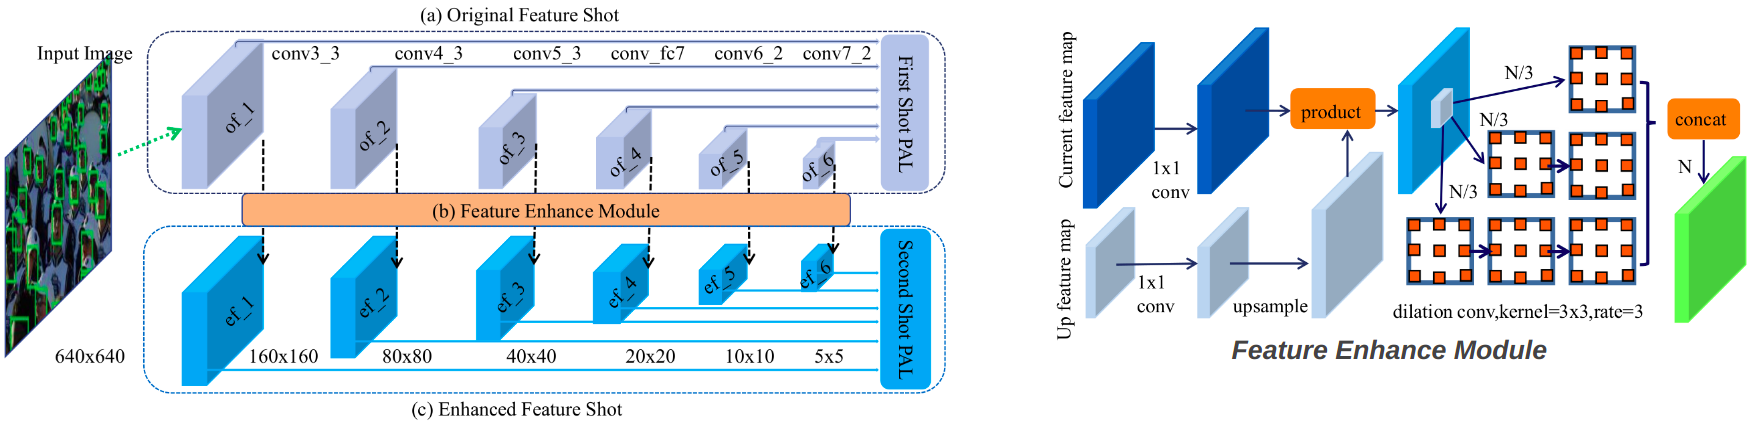
\includegraphics[width=1.0\textwidth]{LiteratureSurvey/DSFD_NN}
    \caption[DSFD]{DSFD NN Architecture}
    \label{fig:dsfdNN} 
\end{figure}

\paragraph{Feature Enhance Module}
Feature Enhance Module shown in figure \ref{fig:dsfdNN} aims to impart wider context information to the network to better detect faces, particularly at small scales. For each feature map, the feature map at the next level is upsampled and integrated with the current feature map. Since the features at the next level have a larger receptive field, this increases the context information available to the current feature map. Finally, a dilated convolution is applied on top of this integrated feature map which further helps to increase the receptive field at the current level as depicted in figure \ref{fig:dilatConvIncRF}.

\begin{figure}[h]
  \centering
    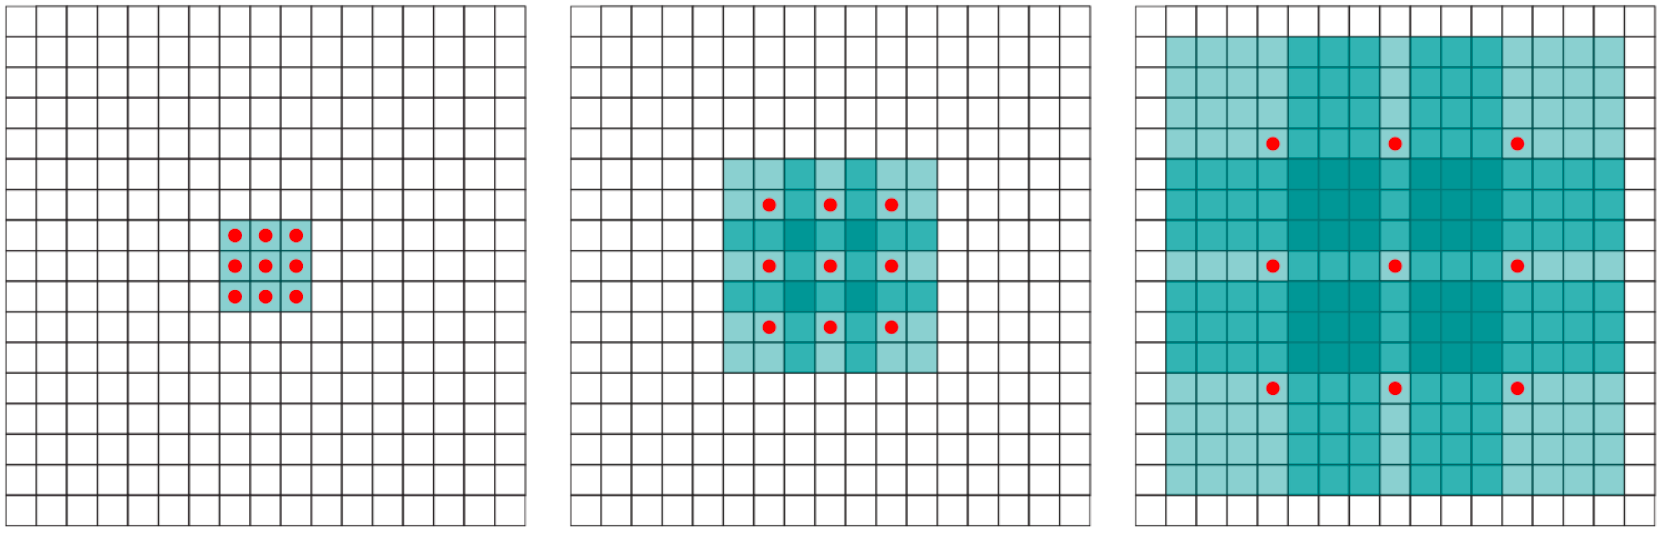
\includegraphics[width=0.7\textwidth]{LiteratureSurvey/DilatConvIncRF}
    \caption[Dilated Convolution]{Increased Receptive Field due to Dilated Convolution}
    \label{fig:dilatConvIncRF} 
\end{figure}


%%%%%%%%%%
\section{LFFD: Light and Fast Face Detector}
As the name suggests, Light and Fast Face Detector \cite{lffd2019} is designed to be a fast real-time face detector with a lightweight model for direct deployment on edge devices that have limited memory storage and low computing power. LFFD is inspired by the single-stage, and multi-scale object detection method SSD \cite{ssd2016}, which also enlightens some other face detectors. One of the characteristics of SSD is that pre-defined anchor boxes are manually designed for each detection branch. These boxes always have different sizes and aspect ratios to cover objects with different scales and shapes. Therefore, anchors play an important role in most single-stage detection methods. However, anchor-based methods may face three challenges:
\begin{enumerate}
    \item Anchor matching is unable to sufficiently cover all face scales. Although this can be relieved, it remains a problem.
    \item Matching anchors to ground-truth bounding boxes is determined by thresholding IoU. The threshold is set empirically, and it is difficult to make a solid investigation of its impact.
    \item Setting the number of anchors for different scales depends on experiences, which may induce sample imbalance and redundant computation.
\end{enumerate}

\paragraph{Anchor-free method}
The key idea is that the Receptive Field (RF) serves as a natural anchor at each detection layer. RF can easily handle the above challenges. Firstly, continuous scales of faces can be predicted within a certain RF size rather than discrete scales in anchor-based methods. Secondly, the matching strategy is clear; namely, an RF is matched to a ground-truth bounding box if and only if its center falls in the ground-truth bounding box. Thirdly, the number of RFs is naturally fixed, and they are regularly distributed in the input image.

Using RFs as anchors naturally raises the concern that faces of different sizes need different RF strategies: for tiny or small faces, Effective Receptive Field (ERF) should cover faces as well as sufficient context information, whereas for large faces, keeping faces in RF is enough, as depicted in figure \ref{fig:RFasAnchor}.

\begin{figure}[h]
  \centering
    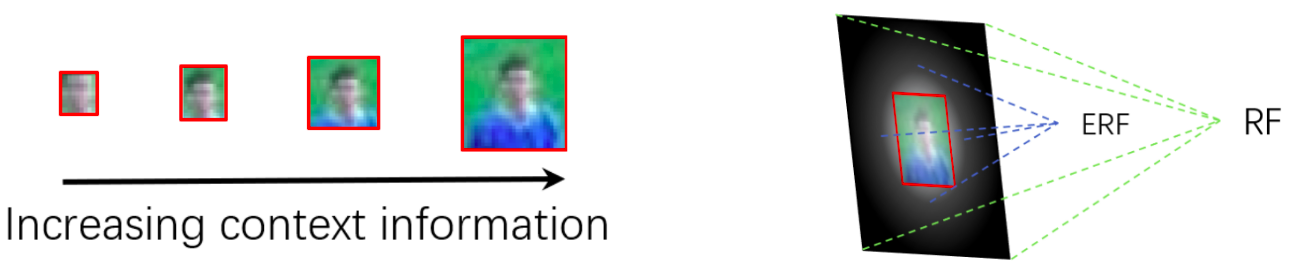
\includegraphics[width=1.0\textwidth]{LiteratureSurvey/RFasAnchor}
    \caption[Receptive Field as Anchor]{Receptive Fields as natural Anchors}
    \label{fig:RFasAnchor} 
\end{figure}


%%%%%%%%%%
\section{YOLOv5 Face}
The YOLO-based object detectors are excellent in real-time detection at high accuracy, which are utilized in many works. YOLOv5 Face Detector \cite{yolov5face2021} is based on the YOLOv5 object detector, with the redesign of some components targeted for face detection. A landmark regression module is added in the object prediction head, lightweight ShuffleNetV2 architecture is used as the backbone to reduce computations, kernel size and stride are modified for some network blocks, and data augmentation methods are optimized, specifically suited for face detection.

There is a portfolio of three YOLOv5 Face detection models available for a variety of trade-offs between speed and accuracy: small, medium, and large. Since the focus of our work is to obtain the best face detector on our dataset instead of real-time application, we run the medium and large models on our dataset.


%%%%%%%%%%
\section{Retina Face}
The key idea of the Retina Face detector \cite{retinaFace2020} is similar to YOLOv5 Face detector, i.e., incorporation of facial landmark regression with the face detection module. But Retina Face takes this idea a step further, and the network is trained for three tasks simultaneously: face bounding box, 2D facial landmarks, and 3D mesh vertices. The method uses ground-truth 3D mesh vertices (figure \ref{fig:RF_mesh}) for multi-task learning. This is a very powerful reinforcement technique since the underlying target for all tasks above is the same: accurate point prediction on the image plane, therefore each task benefits from other tasks, as shown in figure \ref{fig:RF_multiTaskBenefit}

\begin{figure}[h]
    \centering
    \captionsetup[subfigure]{justification=centering}
    \subfloat[Mesh68 and Mesh1k]{{
        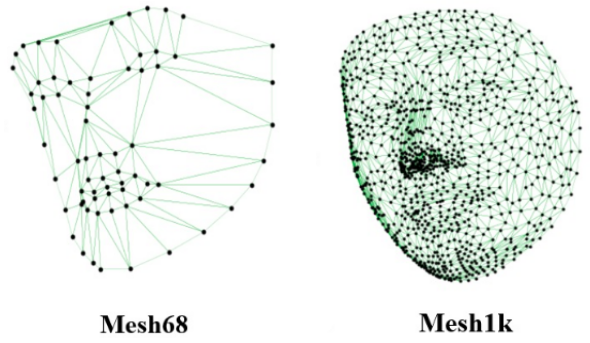
\includegraphics[scale=0.25]{LiteratureSurvey/RF_mesh}
        \label{fig:RF_mesh}
        }}
    \quad
    \subfloat[Multi-task benefit]{{
        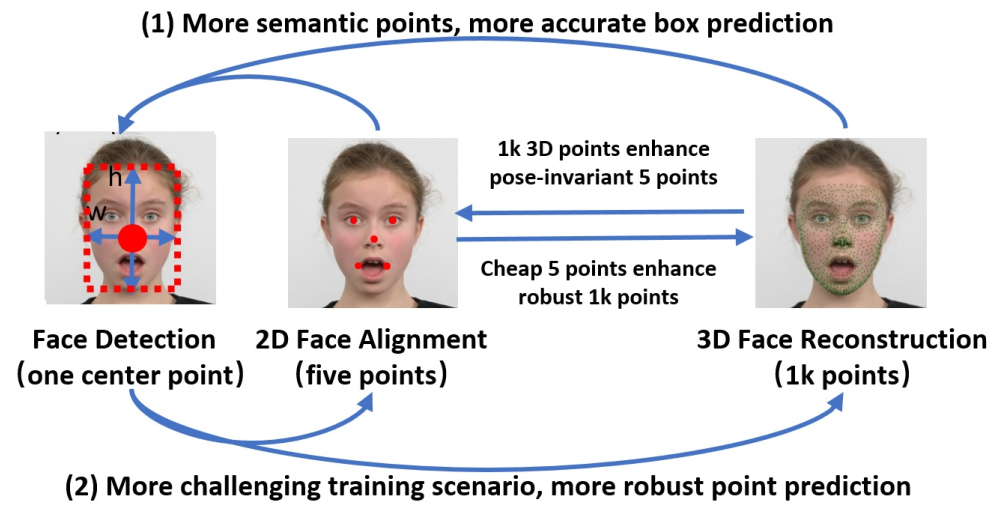
\includegraphics[scale=0.25]{LiteratureSurvey/RF_multiTaskBenefit}
        \label{fig:RF_multiTaskBenefit}
    }}
    \caption{Retina Face}
\end{figure}


%%%%%%%%%%
\section{Menpo 2D and 3D Benchmark}
The Menpo 2D and Menpo 3D benchmarks \citep{menpo} are datasets for multi-pose 2D and 3D facial landmark localization and tracking. In the Menpo 2D benchmark, different visible landmark configurations are designed for semi-frontal and profile faces, thus making the 2D face alignment full pose. In the Menpo 3D benchmark, a united landmark configuration is designed for both semi-frontal and profile faces based on the correspondence with a 3D face model, thus making face alignment not only full-pose but also corresponding to the real-world 3D space.

There are four different types of landmark configurations adopted in the dataset:
\begin{enumerate}
    \item Semi-frontal 2D landmarks: They correspond to the traditional facial landmarks as typically used in the literature. This configuration consists of 68 landmarks.
    \item Profile 2D landmarks: These are specially designed for profile faces where the traditional 2D landmarks are not suitable because a large number of landmarks are self-occluded. This configuration consists of 39 landmarks.
    \item 3DA-2D (3D Aware 2D) landmarks: They are defined as the 2D projections of the 3D landmarks on the image plane. This configuration consists of 84 landmarks.
    \item 3D landmarks: These are defined as the 3D coordinates of the facial landmarks; therefore, they bare information regarding the depth of the 3D face. This configuration consists of 84 landmarks.
\end{enumerate}

\begin{figure}[h]
    \centering
    \captionsetup[subfigure]{justification=centering}
    \subfloat[Semi-frontal 2D landmarks]{{
        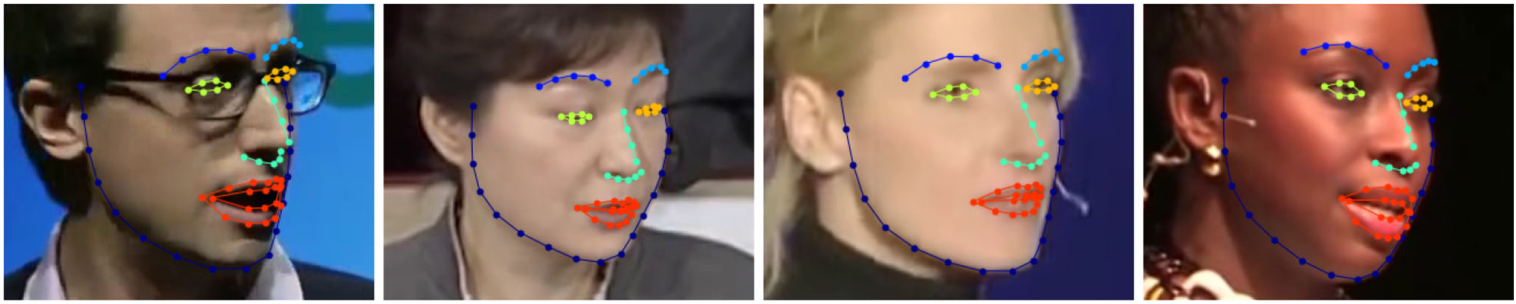
\includegraphics[scale=0.25]{LiteratureSurvey/Semi-frontal_2D}
        \label{fig:semi-frontal_2D}
        }}
    \quad
    \subfloat[3DA-2D landmarks]{{
        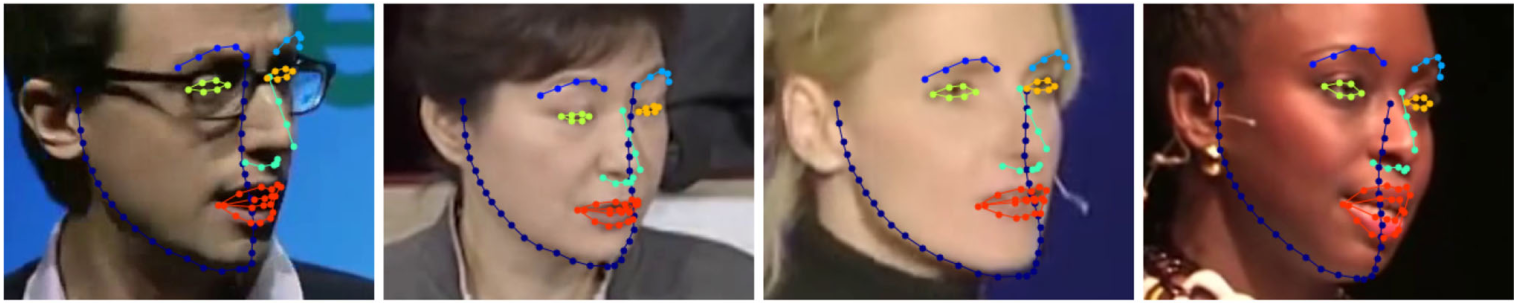
\includegraphics[scale=0.25]{LiteratureSurvey/3DA-2D}
        \label{fig:3DA-2D}
    }}
    \caption[Menpo: Semi-frontal 2D and 3DA-2D landmarks]{Menpo: Comparison of Semi-frontal 2D and 3DA-2D landmarks}
\end{figure}

\subsection{Ground-Truth creation of 3DA-2D and 3D Facial Landmarks}
Initially, a DCNN network \cite{dcnn} is employed to estimate the per frame 3DA-2D landmarks as a ground truth. Then, an energy minimization method is used to fit the combined identity and expression models on the landmarks of all frames of the video simultaneously. In more detail, a 3D Morphable Model is utilized as an identity and expression model. The vertices of these mesh models are rotated and translated using a linear view transformation to bring them into the camera reference frame:

\begin{equation}
\mathbf{v} = [v_x, v_y, v_z]^T = \mathbf{R}_v \mathbf{x} + \mathbf{t}_v
\end{equation}

where $\mathbf{R}_v$ and $\mathbf{t}_v$ are the camera's 3D rotation and translation components, respectively. Then, the camera projection is applied. For the sake of computational efficiency and stability, a scaled orthographic camera is considered, i.e., the 2D location of the 3D point $\mathbf{x}'$ is given by:

\begin{equation}
\mathbf{x}' = \sigma [v_x, v_y]^T
\end{equation}

where $\sigma$ is the scale parameter of the orthographic camera. Then, an optimization method using energy minimization is used to fit the obtained 2D coordinates to obtain the parameters of the model.


%%%%%%%%%%
\section{Comparison of Face Detectors}
The input face and eyes have to be extracted before they can be fed to the neural network. We explored several face detectors, as discussed in above sections, in order to figure out the best extractor. Precision-Recall curves and Average Precision (AP) scores are widely used as standard metrics to compare object detection algorithms (the face being the object in this work).

Precision measures the ability of a model to detect the true positives (i.e., faces) with high accuracy and low error. It is defined as the ratio of true positives to all the positive detections reported by the model. Recall is the ability of the model to detect all the the true positives present in the data. It is defined as the ratio of true positives to the sum of true positives and false negatives. The Precision-Recall curve is often plotted to negotiate a trade-off between the precision and recall values of a detection model. The area under the Precision-Recall curve quantifies this trade-off, which is called the Average Precision (AP) score of the model.

\begin{equation}
\begin{split}
Precision & = \frac{TP}{TP + FP} \\
Recall & = \frac{TP}{TP + FN}
\end{split}
\end{equation}
where,

\quad TP = True Positives

\quad FP = False Positives

\quad FN = False Negatives

Figure \ref{fig:result_allDetectors} compares the precision-recall curves of various detectors discussed in earlier chapter. From these results, it can be seen that DSFD works the best on our dataset, with the highest AP score at various IoU thresholds. Other detectors like Retina Face, S3FD, and LFFD are competitively accurate with DSFD, and at a reasonable IoU threshold of 0.5 or 0.6, the difference in AP scores is not very significant. But the YOLOv5 Face detector performs the worst among all. A reasonable explanation could be that all others are dedicated face detectors with dedicated pipelines for face detection, whereas YOLOv5 Face is just an extension of the YOLOv5 object detector.

\begin{figure}[h]
    \centering
    \captionsetup[subfigure]{justification=centering}
    \subfloat{{
        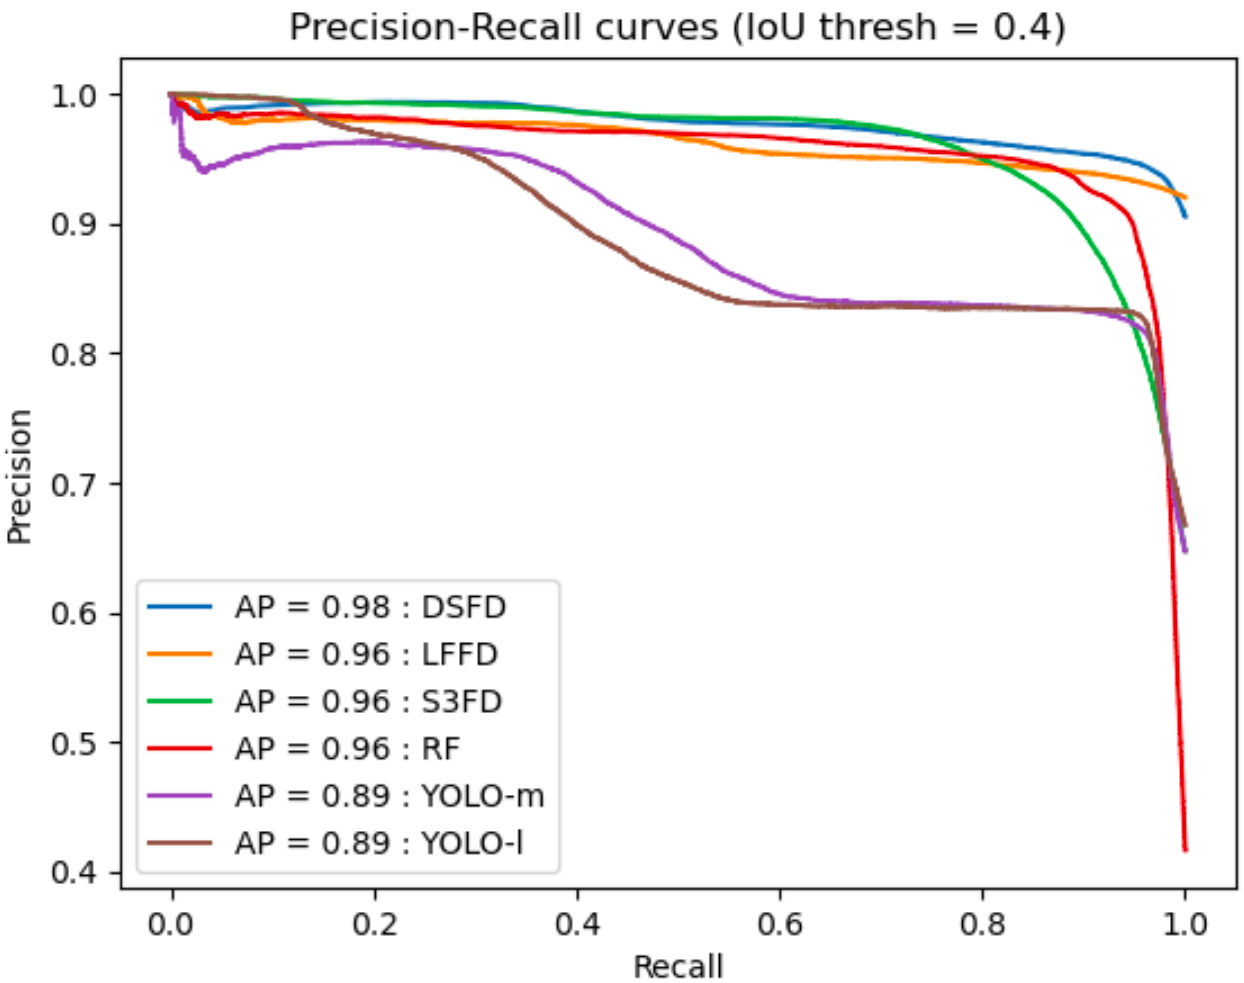
\includegraphics[width=0.45\textwidth]{LiteratureSurvey/DetectorAcc_Thresh-0.4}
        }}
    \quad
    \subfloat{{
        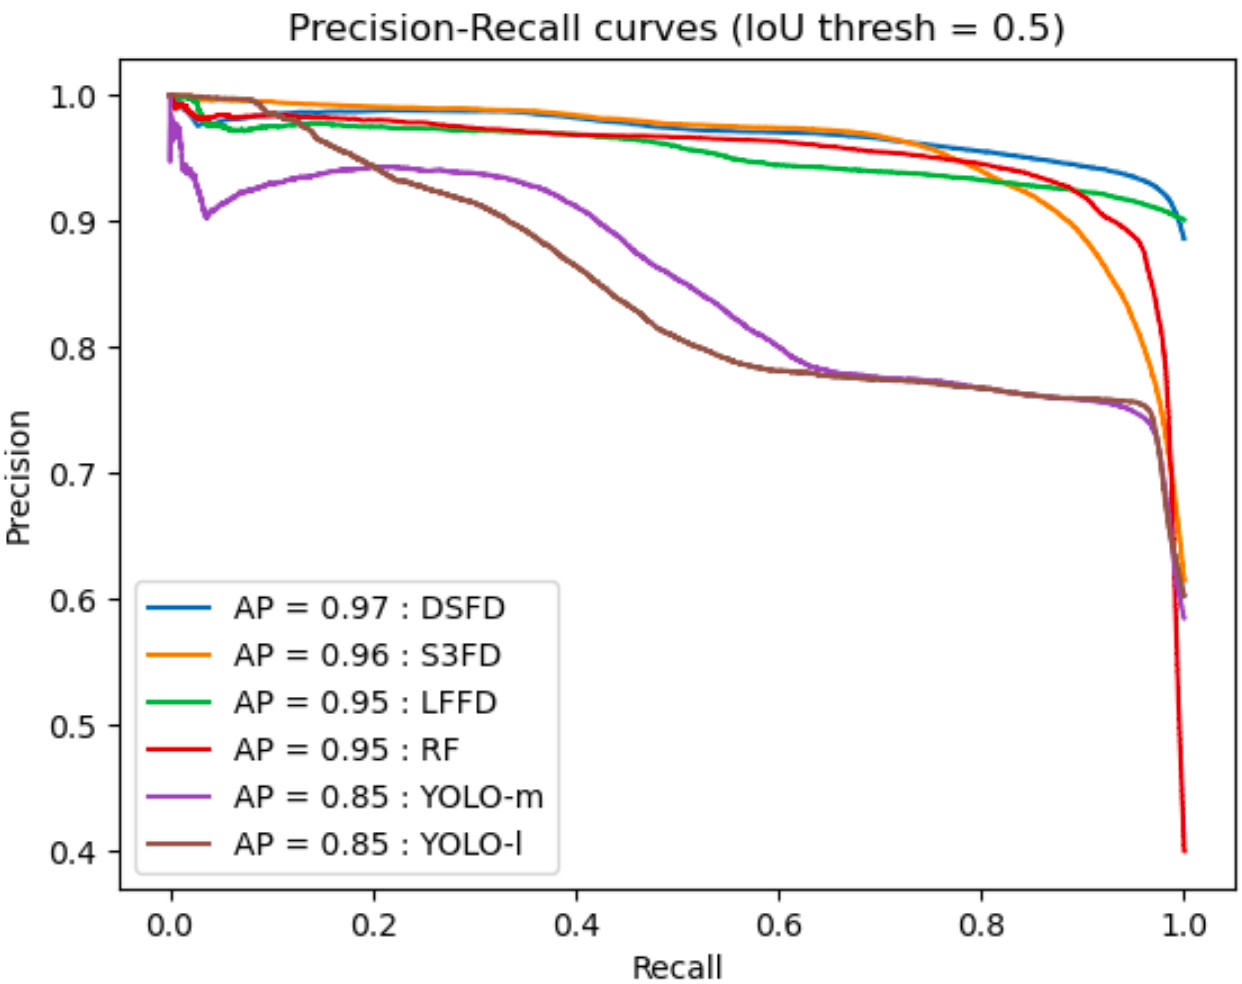
\includegraphics[width=0.45\textwidth]{LiteratureSurvey/DetectorAcc_Thresh-0.5}
    }}
    \quad
    \subfloat{{
        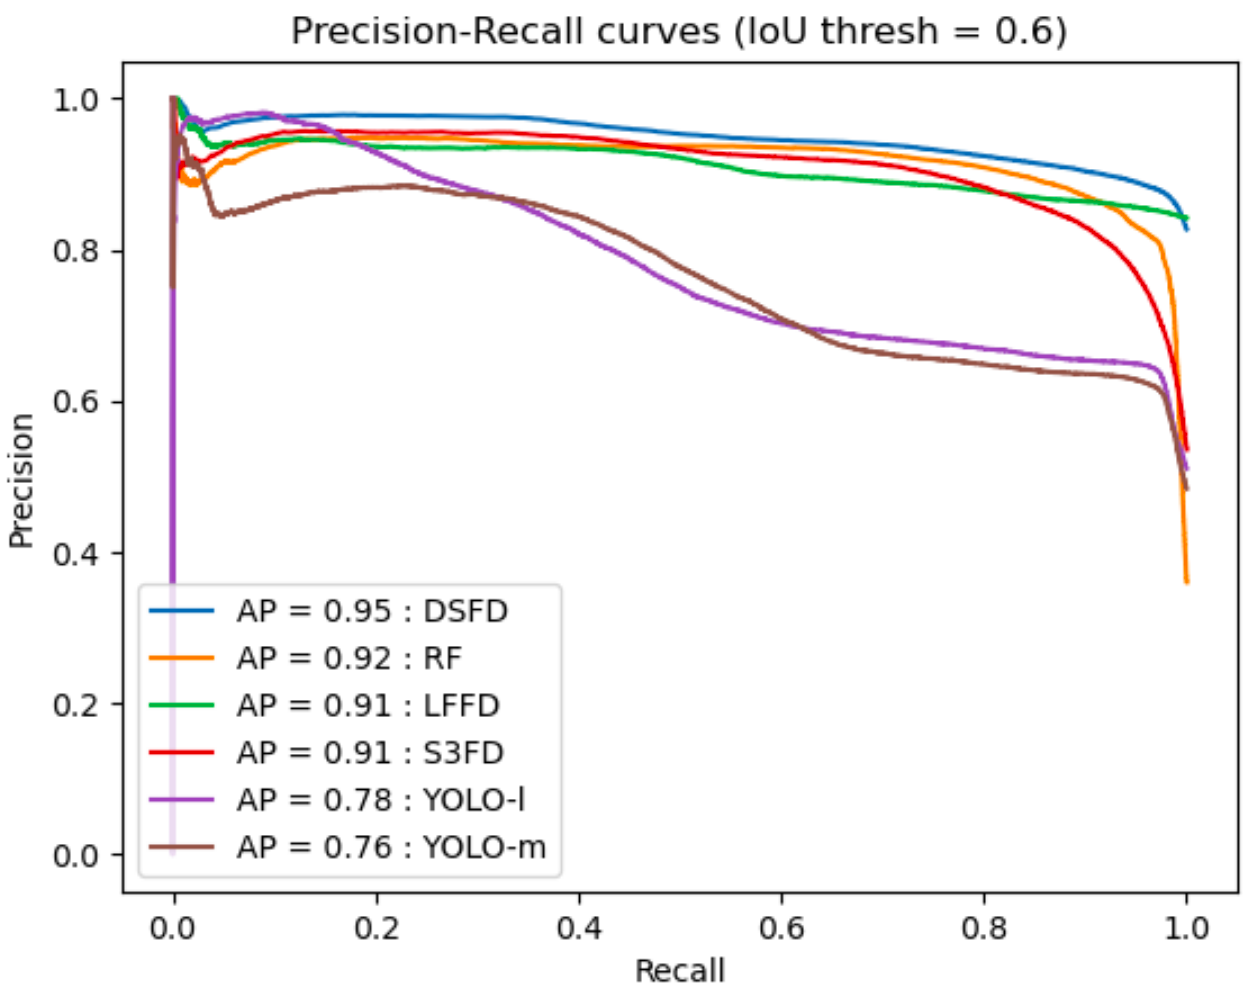
\includegraphics[width=0.45\textwidth]{LiteratureSurvey/DetectorAcc_Thresh-0.6}
    }}
    \quad
    \subfloat{{
        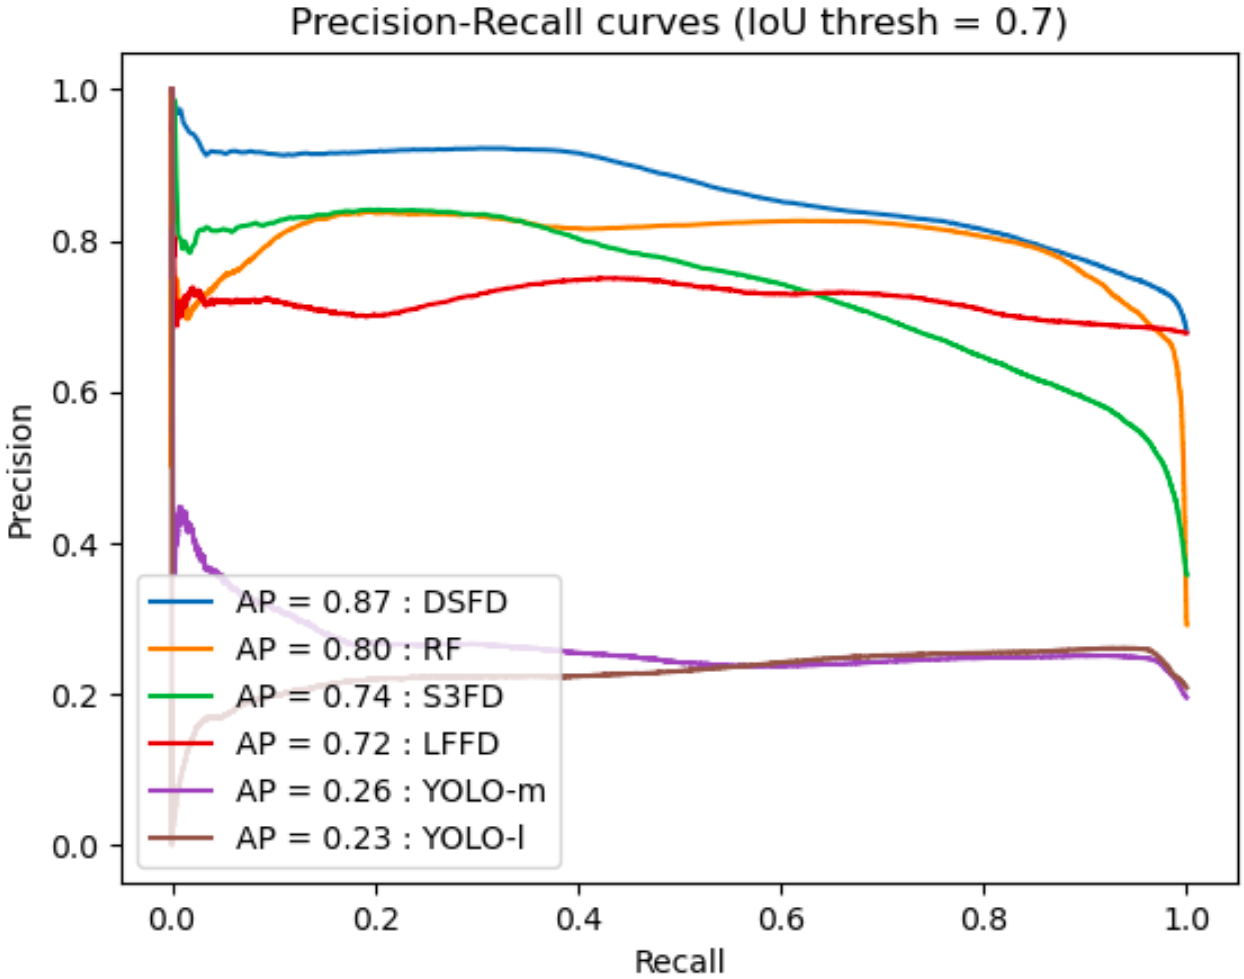
\includegraphics[width=0.45\textwidth]{LiteratureSurvey/DetectorAcc_Thresh-0.7}
    }}
    \caption{Accuracy comparison of various detectors}
    \label{fig:result_allDetectors}
\end{figure}

\begin{figure}[h]
  \centering
    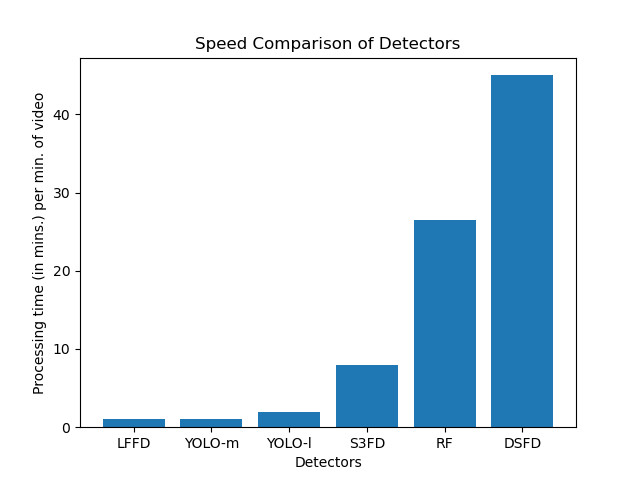
\includegraphics[scale=0.6]{LiteratureSurvey/Result_speed}
    \caption{Speed comparison of various detectors}
    \label{fig:result_speed}
\end{figure}

Out of all detectors used, the speed of DSFD is the slowest, as expected from the study of its architecture. It has a 2-stage pipeline, namely Original Feature Shot and Enhance Feature Shot which increases the runtime of DSFD. On the other hand, YOLOv5 Face and LFFD are the fastest detectors and can be used for real-time face detection applications. For an effective accuracy-speed trade-off, Retina Face is an excellent detector. So, for all extractions in our experiments, we used the Retina Face detector.